\chapter{基于说话人特征的跨语种语音转换优化方法}

\section{引言}

上文介绍了本文提出了基于半优化CycleGAN的非平行语料语音转换系统,该框架可以在一般非平行语料的语音转换任务上
得到较高的音质。然而,当原始说话人和目标说话人两个领域的差距较大时,转换的难度就会显著增加,差距可以体现在
说话人信息,语速,语义,音调等。在这种情况下,转换语音的音质会有明显的下降,甚至会无法训练。另一方面,实际
应用场景中,两个差距较大的领域是比较常见的,之前实验中的数据都是在专业录音环境下录制的平稳朗读语音,属于较为
理想的情况。因此,对领域差距较大情况下的语音转换任务进行优化具有较高的实际应用价值和研究价值。本章将对其中
较为极端的任务作为研究对象,即跨语种的语音转换。在该任务中,两个领域不仅是说话人信息不同,在语义信息上也
具有较大的差异,这对模型性能提出了挑战。

本章提出一种基于说话人特征的跨语种语音转换方法,以第三章介绍的CycleGAN-VC方法为基础,在CycleGAN模型中引入
说话人识别机制。首先需要先训练一个说话人识别模型,之后使用模型中的d-vector提取器来作为CycleGAN中判别器的
前置模型,使得判别器可以只使用说话人信息作为判别标准。实验证明,引入说话人特征的语音转换方法可以有效实现
在保留语义的前提下实现说话人语音转换,有效提升模型性能。

在接下来的内容中,将首先对跨语种语音转换和相关工作进行简要介绍,然后对说话人识别及其相关特征进行说明,
之后将详细介绍本章提出的引入说话人特征的跨语种语音转换优化方法,最后对实验配置及其结果进行分析。

\section{跨语种语音转换}
\subsection{跨语种语音转换概述}
根据转换语言条件的不同,可以将语音转换分为两类:单语种语音转换和跨语种语音转换。在单语种语音转换中,训练集中
原始说话人和目标说话人的语言是相同的,在测试时也是同一种语言。相对的,跨语种语音转换则是原始说话人和目标说话人的
语言不同,在此基础上可以将其再分为两类:一类是原始说话人的训练集是双语种的,其中一个语种和目标说话人一致;另一类
则是完全不相同。早期在跨语种语音转换上的研究多基于第一类情况,在本章我们则将以第二类为研究对象。跨语种语音转换具有较好
的发展和应用前景,作为无监督学习任务,其可以实现让一个不会说某种语言的说话人以他的声音说该语言。在语音翻译中,
通常需要将某个说话人的语音翻译为另一种语言的语音,然而翻译语音通常不是该说话人的声音,跨语种语音转换便可以作为
补充,完善语音翻译的整个环节。

尽管跨语种的语音转换的研究仍处于初步阶段,但研究人员针对跨语种的特点,提出了一些有效的方法。在\cite{AbeStatistical}中,
一个双语种的转换模型在目标语言的平行训练数据上训练,这需要原始说话人的训练数据不仅包含原始语种,也包含目标语种。
然而,事实上双语种说话人的双语数据是较难获得的。因此一些用于在非平行数据中找到对应的原始-目标帧的非平行对齐技术
被开发出来,例如单元选择\cite{sundermann2006text,Hao2015AA}和迭代对齐法\cite{erro2007frame,erro2009inca}。
但是这些方法由于不准确性使得转换性能只处于中等。基于声道长度归一化的音素映射方法也被提出\cite{sundermann2003vtln,qian2011frame},
这些方法中弯折函数是通过原始和目标特征之间最接近的音素或声学类来估计的。研究人员也提出了基于音素后验概率图的方法\cite{sun2016personalized,zhou2019cross},
该方法使用单语种或双语种的音素字典来作为中间的说话人无关特征,实现跨语种的转换。

\subsection{跨语种语音转换的难点}
% 1.不同语种之间文本信息不一致导致较难匹配
% 2.不同语种声学特征差异较大,对cyclegan有挑战性
如前文所述,跨语种语音转换作为一个无监督任务,是非平行语料语音转换的一个特殊任务。相比于通常的非平行语料语音转换,
跨语种语音转换转换难度更大,目前方法的效果也都不尽如人意。主要难度体现在以下两个方面。

\begin{figure}[!htp]
    \centering
    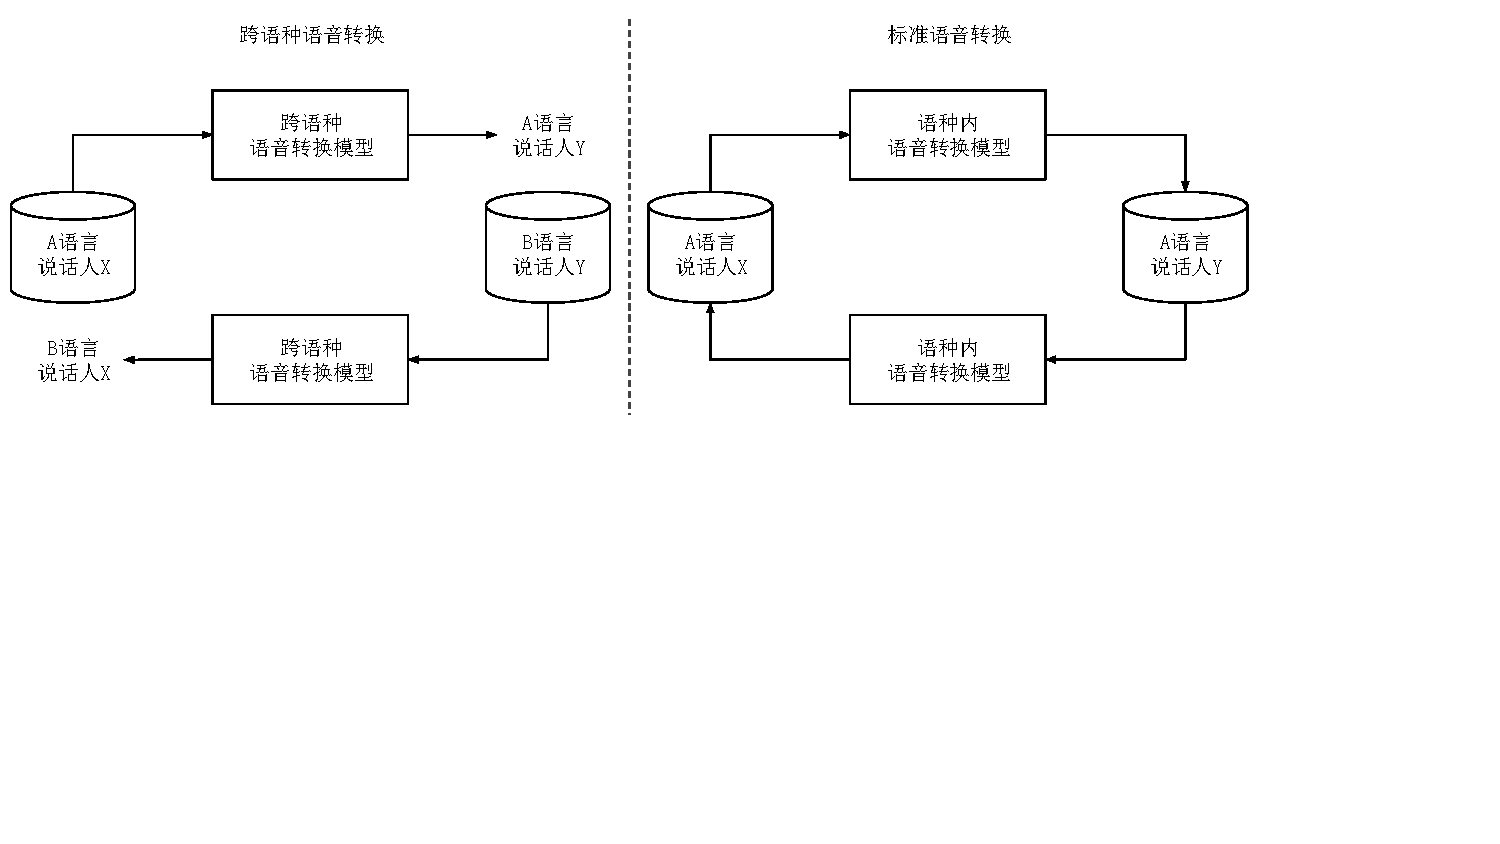
\includegraphics[width=14cm,trim=0 200 80 0,clip]{figure/5_clvc.pdf}
    \bicaption[跨语种语音转换和标准语音转换对比图]
    {跨语种语音转换和标准语音转换对比图}
    {Comparison of cross-lingual Voice Conversion and standard Voice Conversion}
    \label{fig:clvc}
\end{figure}

\begin{itemize}
    \item 不同语种之间文本信息不一致导致较难匹配。由于跨语种的语音转换涉及到两种不同的语言,因此平行语料的语音转换方法将完全不适用。
    另一方面若使用非平行的对齐方法,语种之间的巨大差异也会导致对齐准确度的下降。因此如何找到有效的单元匹配方式或无监督的训练方式是
    跨语种语音转换面临的主要挑战。
    \item 差异较大的声学特征与CycleGAN训练机制的矛盾。该矛盾分为两个方面。如前文所述,CycleGAN之所以能够实现语音转换任务,判别器在其中有着关键的作用。
    判别器在训练时,会分别输入正例和负例,对应训练标签$1$和$0$,其中正例是目标说话人的真实特征序列,负例是从原始说话人声学特征经
    生成器转换的目标说话人的转换特征序列,判别器的目标是尽可能地区分正例和负例。生成器在训练时会将生成的目标说话人转换特征传递给判别器,
    并将判别器的判别结果与$1$计算损失,来衡量转换特征和真实目标特征之间的差距,然后将梯度回传给生成器,这样生成器下次在遇到类似输入时,
    就会生成更接近判别器正例的转换特征。从图\ref{fig:clvc}中可以注意到,在跨语种语音转换中,判别器的正例
    是目标语种的目标说话人特征序列,而负例是原始语种的目标说话人特征序列。当判别器尝试区分正负例时,总是会尝试以区分度最大的信息作为
    判别要素,此时当语种信息的差异化大于说话人信息的差异化时,判别器就会转变为一个语种分类器,进而导致生成器无法从判别器中得到正确的
    梯度,因此在基线试验中,经常会导致模型在训练时无法训练成功:输入中文,生成器会输出无意义的英文语音。另一方面,语种的差异也会导致
    跨语种语音转换没有一个标准的对偶任务。如图\ref{fig:clvc}中左图所示,主任务为将说话人X的A语言转为说话人Y的A语言,理论上对偶任务
    应是说话人Y的A语言转为说话人X的A语言,而实际上对偶任务则是说话人Y的B语言转为说话人X的B语言。这样的不完全对偶性也增加了CycleGAN在
    跨语种语音转换任务上的难度。
\end{itemize}


\section{说话人识别}
\subsection{说话人识别概述}
\subsection{d-vector说话人特征}

\section{引入说话人特征的跨语种语音转换}
\subsection{语种无关的d-vector提取器训练}
\subsection{d-vector提取器和CycleGAN的结合}

\section{实验分析}
% 客观指标可以用d-vector的距离来判断
% 引入说话人特征的有效性:
% 主观实验-自然度,相似度
% 系统:
% 1. baseline, 标准CycleGAN
% 2. 加入d-vector(d-vector 512, 100人)
% 3. 加入d-vector(d-vector 64, 100人)
% 4. 加入d-vector(d-vector 64, 1000人)
% 客观实验:
% 测试接上转换特征d-vector和目标特征的差距
% cycle-consistency loss
\subsection{实验配置}
\subsection{引入说话人特征的有效性检验}
\subsection{说话人分类模型的比较}


\section{本章小结}